\chapter{Techniques de laboratoire II~: synthèse et analyse en pratique}\label{ch:b2:lab-techniques-2}

Une réaction de Grignard échoue un lundi matin~: le ballon avait été rincé mais pas séché, et les
quelques gouttes d'eau restées dedans ont détruit le réactif à mesure qu'il se formait. Reprise dans une
verrerie séchée à l'étuve, sous diazote, l'halogénure étant ajouté goutte à goutte dans un ballon agité
et refroidi, la même réaction fonctionne. La chimie n'a pas changé~; le montage, si. Ce chapitre traite
de la pratique qui transforme une réaction sur le papier en un produit dans un flacon~: maîtriser la
réaction, tenir l'air et l'eau à l'écart, la traiter, purifier le produit et prouver ce qu'on a obtenu.

\begin{omfigure}
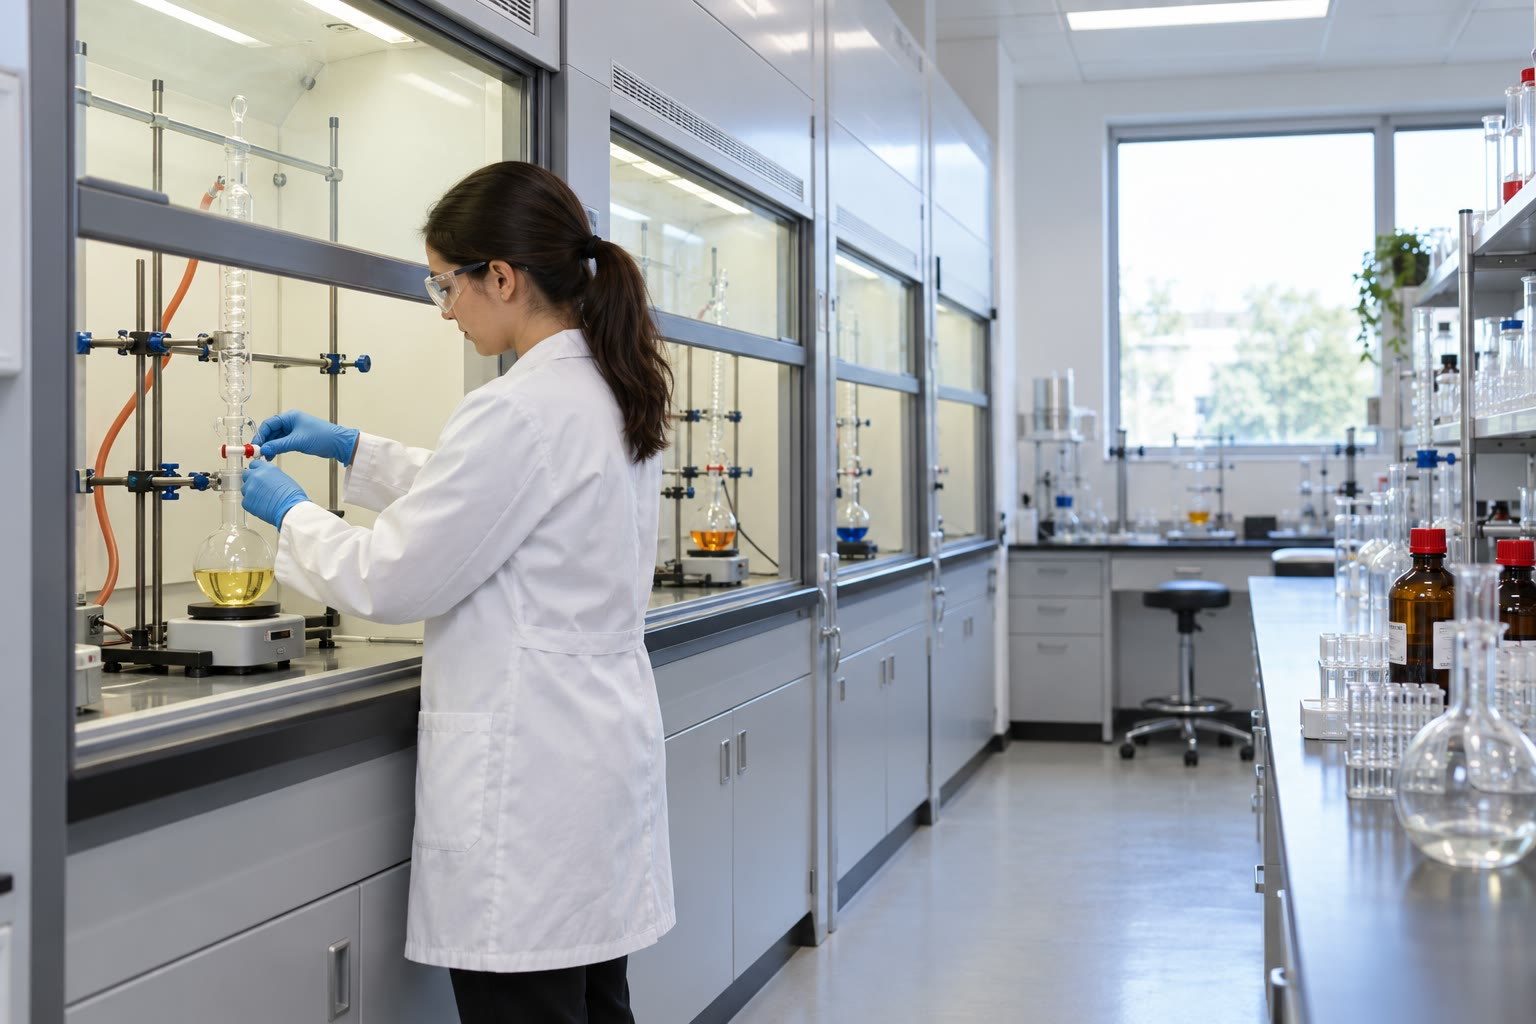
\includegraphics[width=0.56\linewidth]{images/book3/ai/b2-35-synthesis-lab.jpg}

{\small Un laboratoire de synthèse organique~: réactions menées sous hotte, ballons fixés sur des
potences (illustration).}
\end{omfigure}

\begin{recall}
Le volume de première année~: dangers et étiquetage SGH, extraction, recristallisation, distillation,
\omterm{def:b2:chromatography:principle}{chromatographie} sur couche mince et $R_f$, température de fusion, organomagnésiens.
\Cref{ch:b2:reaction-enthalpy}~: \omterm{def:b2:reaction-enthalpy:reaction-quantity}{enthalpie de réaction} et \omterm{def:b2:continuous-reactors:adiabatic-rise}{élévation adiabatique de température}.
\Cref{ch:b2:chromatography},
\cref{ch:b2:structure-determination} et \cref{ch:b2:measurement-statistics}~: analyse.
\end{recall}

\section{Conduire une réaction sous contrôle}

Une réaction dans un ballon libère sa chaleur là où elle se produit. Le chimiste maîtrise la
température par un bain (eau et glace, glace et sel, carboglace et acétone pour les plus basses
températures), par le reflux d'un solvant à ébullition, qui plafonne la température à sa température
d'ébullition tandis que le réfrigérant renvoie la vapeur, et par la vitesse d'ajout d'un réactif. Un
thermomètre interne, plongé dans le liquide plutôt que dans le bain, mesure ce qui compte.

\begin{proposition}[Accumulation]\label{prop:b2:lab-techniques-2:accumulation}
Si un réactif est ajouté plus vite qu'il ne réagit, la quantité qui n'a pas réagi, $n_{\mathrm{acc}}$,
s'accumule. Si elle réagit ensuite d'un seul coup, sans refroidissement, la température du mélange, de
capacité thermique $C$, s'élève de
\begin{equation*}
\Delta T_{\mathrm{ad}} = \frac{n_{\mathrm{acc}}\,|\Delta_rH|}{C}.
\end{equation*}
\end{proposition}

\begin{proof}
La réaction de $n_{\mathrm{acc}}$ libère $n_{\mathrm{acc}}|\Delta_rH|$ à pression constante
(\cref{ch:b2:reaction-enthalpy})~; sans échange thermique, toute cette énergie échauffe le mélange, comme
pour la \omterm{def:b2:reaction-enthalpy:flame-temperature}{température de flamme adiabatique} (\cref{def:b2:reaction-enthalpy:flame-temperature})~: $C\Delta T =
n_{\mathrm{acc}}|\Delta_rH|$.
\end{proof}

Le danger est maximal quand une réaction tarde à démarrer, comme c'est souvent le cas pour la formation
des organomagnésiens~: l'halogénure ajouté avant l'amorçage s'accumule, et quand la réaction démarre
enfin, elle s'emballe. La règle est d'ajouter une petite portion, de voir la réaction démarrer
(échauffement, trouble, léger reflux), et seulement ensuite d'ajouter le reste au rythme que le
refroidissement peut suivre.

\section{Conditions anhydres et atmosphère inerte}

\begin{definition}[Atmosphère inerte]\label{def:b2:lab-techniques-2:inert}
On conduit une réaction sous \emph{atmosphère inerte}\index{atmosphere inerte@atmosphère inerte} quand
l'air de l'appareil a été remplacé par un gaz qui ne réagit pas, le diazote ou l'argon, maintenu en
légère surpression pour que l'air ne puisse pas entrer.
\end{definition}

Les réactifs organométalliques, les hydrures métalliques et de nombreux catalyseurs réagissent avec
l'eau et le dioxygène. La verrerie est séchée à l'étuve et montée chaude, ou flambée sous courant de
gaz~; les solvants sont achetés anhydres ou séchés sur un réactif qui réagit avec l'eau~; les liquides
sont transférés à la seringue à travers des septums en caoutchouc. Le gaz sort par un barboteur à huile,
qui montre le débit et empêche l'air de refluer. La rampe de Schlenk et la boîte à gants, pour les
composés les plus sensibles, sont présentées dans le volume de troisième année.

\begin{omfigure}
\begin{tikzpicture}[lab/.style={font=\scriptsize, align=center}]
\fill[omDef!10] (-1.7,-0.3) rectangle (1.7,1.0);
\draw[om glass] (-1.7,1.2) -- (-1.7,-0.3) -- (1.7,-0.3) -- (1.7,1.2);
\foreach \x/\y in {-1.5/0.0,-1.45/0.55,1.3/0.05,1.3/0.6,-1.25/0.3,1.05/-0.15}{
  \draw[omDef!50, fill=white] (\x,\y) rectangle ++(0.18,0.18);}
\pic (f) at (0,0) {threeneck={0.35}{omThm!25}};
\pic[rotate=25] (d) at (f-l) {dropfunnel={0.5}{omMeth!20}};
\pic (c) at (f-c) {condenser};
\pic[rotate=-25] (t) at (0.0,0.42) {thermometer};
\pic (b) at (3.6,3.6) {bubbler};
\draw[thick, black!60] (0,6.25) -- (0,6.75) -- (3.25,6.75) -- (b-in);
\coordinate (dtop) at ($(f-l)+(-1.52,3.26)$);
\draw[thick, black!60] (dtop) -- ++(0,0.35) -- ++(-0.9,0) node[left, lab] {N$_2$};
\node[lab, anchor=north] at (0,-0.4) {bain de glace};
\node[lab, anchor=east] at (-1.9,2.6) {ampoule\\de coulée};
\node[lab, anchor=west] at (0.55,5.0) {réfrigérant};
\node[lab, anchor=west] at (1.75,2.6) {thermomètre\\(interne)};
\node[lab, anchor=north] at (3.6,3.45) {barboteur (sortie de gaz)};
\end{tikzpicture}
\par\vspace{4pt}

{\small Une réaction sous diazote (schéma). Ballon tricol dans un bain de glace, avec un thermomètre
interne plongé dans le liquide~; le réactif est ajouté à partir d'une ampoule de coulée isobare par
laquelle entre le diazote~; le gaz sort par le réfrigérant et un barboteur à huile.}
\end{omfigure}

\begin{method}[Monter une réaction anhydre sous diazote]\label{met:b2:lab-techniques-2:anhydrous}
\begin{enumerate}
  \item Sécher la verrerie à l'étuve et la monter chaude, en graissant les rodages ou en les équipant de
        manchons~; mettre en place un septum ou l'ampoule de coulée, le réfrigérant et le barboteur.
  \item Balayer au diazote pendant le refroidissement~; maintenir un faible débit (une bulle toutes les
        une à deux secondes) pendant toute l'opération.
  \item Introduire les solides avant le balayage, les solvants anhydres et les réactifs liquides à la
        seringue ou à la canule à travers un septum.
  \item Refroidir ou chauffer comme prévu~; commencer l'ajout par une petite portion et vérifier que la
        réaction démarre avant de poursuivre.
\end{enumerate}
\end{method}

\section{Traitement}

\begin{definition}[Traitement]\label{def:b2:lab-techniques-2:work-up}
Le \emph{traitement}\index{traitement d'une reaction@traitement d'une réaction} d'une réaction est la
suite d'opérations qui, une fois la réaction terminée, transforme le mélange réactionnel en produit
brut~: hydrolyse des réactifs restants, extraction et lavages, séchage, filtration et évaporation du solvant.
\end{definition}

\begin{definition}[Extraction acide--base]\label{def:b2:lab-techniques-2:acid-base-extraction}
Une \emph{extraction acide--base}\index{extraction acide--base} sépare des composés organiques acides,
basiques et neutres dissous dans un solvant organique en lavant la solution par des acides ou des bases
en solution aqueuse, qui transforment une classe de composés en ions qui passent dans l'eau.
\end{definition}

\begin{proposition}[Qui va où]\label{prop:b2:lab-techniques-2:acid-base-extraction}
L'hydrogénocarbonate de sodium aqueux (pH 8.3) extrait un acide carboxylique ($\mathrm pK_a$ vers 4)
mais pas un phénol ($\mathrm pK_a$ vers 10), qui exige l'hydroxyde de sodium~; l'acide chlorhydrique
dilué extrait une amine dont l'acide conjugué a un $\mathrm pK_a$ de 4.6 ou plus~; les composés neutres
restent dans la phase organique.
% ledger: ph:NaHCO3, pka:benzoic, pka:phenol, pka:anilinium
\end{proposition}

\begin{proof}
Une espèce est surtout sous sa forme basique quand $\mathrm{pH} > \mathrm pK_a$, et à plus de 99~\% quand
$\mathrm{pH} > \mathrm pK_a + 2$. À pH 8.3, l'acide benzoïque (4.2) est à plus de 99~\% sous forme de
benzoate, un ion qui reste dans l'eau~; le phénol (9.99) n'est qu'à environ 2~\% sous forme de phénolate
($10^{8.3 - 10.0}$) et reste pour l'essentiel dans la phase organique, où se partage la forme neutre.
Dans l'hydroxyde de sodium (pH supérieur à 12), le phénol est transformé en phénolate. Dans l'acide
chlorhydrique dilué (pH voisin de 1), l'aniline (anilinium 4.6) est à plus de 99~\% sous forme
d'anilinium. Chaque ion, une fois dans l'eau, est récupéré en ramenant le pH dans l'autre sens, ce qui
régénère le composé neutre, puis en l'extrayant de nouveau.
\end{proof}

\begin{omfigure}
\begin{tikzpicture}[x=1cm, y=1cm, st/.style={draw=black!70, rounded corners=2pt, fill=white,
  font=\scriptsize, align=center, inner sep=3pt, text width=3.0cm}, ar/.style={->, thick, black!70}]
\node[st, fill=omDef!10] (m) at (0,0) {acide benzoïque,\\phénol, aniline,\\naphtalène dans\\l'éthoxyéthane};
\node[st, fill=omThm!10] (a1) at (5.0,0) {aqueuse~: benzoate\\$\to$ HCl $\to$ acide benzoïque};
\node[st] (o1) at (0,-1.6) {phénol, aniline,\\naphtalène};
\node[st, fill=omThm!10] (a2) at (5.0,-1.6) {aqueuse~: phénolate\\$\to$ HCl $\to$ phénol};
\node[st] (o2) at (0,-3.2) {aniline, naphtalène};
\node[st, fill=omThm!10] (a3) at (5.0,-3.2) {aqueuse~: anilinium\\$\to$ NaOH $\to$ aniline};
\node[st, fill=omMeth!10] (o3) at (0,-4.8) {naphtalène\\(sécher, évaporer)};
\draw[ar] (m) -- node[above, font=\tiny] {NaHCO$_3$} (a1);
\draw[ar] (m) -- (o1); \draw[ar] (o1) -- node[above, font=\tiny] {NaOH} (a2);
\draw[ar] (o1) -- (o2); \draw[ar] (o2) -- node[above, font=\tiny] {HCl} (a3);
\draw[ar] (o2) -- (o3);
\pic at (8.6,-3.6) {sepfunnel={omDef!25}{omThm!20}};
\node[font=\scriptsize, align=center] at (8.6,-4.0) {ampoule à décanter};
\end{tikzpicture}
\par\vspace{4pt}

{\small Séparation acide--base de quatre composés (\cref{prop:b2:lab-techniques-2:acid-base-extraction}).
La phase organique (colonne de gauche) perd une classe à chaque lavage~; chaque extrait aqueux (à
droite) rend son composé quand on inverse le pH.}
\end{omfigure}

\begin{definition}[Agent desséchant]\label{def:b2:lab-techniques-2:drying-agent}
Un \emph{agent desséchant}\index{agent dessechant@agent desséchant} est un sel anhydre, comme le sulfate
de magnésium ou de sodium, qui fixe l'eau dissoute dans une solution organique sous forme d'eau
d'hydratation et qu'on élimine ensuite par filtration.
\end{definition}

\begin{method}[Du ballon réactionnel au produit brut]\label{met:b2:lab-techniques-2:work-up}
\begin{enumerate}
  \item Hydrolyser~: détruire les réactifs réactifs restants par une solution aqueuse adaptée, lentement
        et en refroidissant.
  \item Extraire par un solvant organique~; séparer les phases (vérifier laquelle est laquelle en ajoutant
        une goutte d'eau)~; extraire de nouveau la phase aqueuse.
  \item Laver les phases organiques réunies (acide, base, puis saumure, solution saturée de chlorure de
        sodium qui retire l'essentiel de l'eau dissoute).
  \item Sécher par un \omterm{def:b2:lab-techniques-2:drying-agent}{agent desséchant} jusqu'à ce qu'une partie reste pulvérulente~; filtrer.
  \item Éliminer le solvant à l'évaporateur rotatif sous pression réduite~; peser le produit brut.
\end{enumerate}
\end{method}

\section{Purification}

\begin{definition}[Chromatographie flash]\label{def:b2:lab-techniques-2:flash}
La \emph{chromatographie flash}\index{chromatographie flash} est une \omterm{def:b2:chromatography:principle}{chromatographie} préparative sur
colonne de silice dans laquelle l'éluant est poussé à travers la colonne par une légère pression de gaz,
si bien que la séparation de quelques grammes de matière prend quelques minutes~; l'éluant est choisi par
\omterm{def:b2:chromatography:principle}{chromatographie} sur couche mince sur la même silice.
\end{definition}

\begin{proposition}[Volumes de colonne]\label{prop:b2:lab-techniques-2:column-volumes}
Un composé qui migre avec un $R_f$ donné sur une plaque de CCM sort d'une colonne de la même silice et
du même éluant après environ $1/R_f$ volumes de colonne d'éluant.
\end{proposition}

\begin{proof}[Argument]
Sur la plaque, le composé parcourt $R_f$ fois la distance du front de solvant~: sa vitesse moyenne vaut
$R_f$ fois celle de l'éluant. Dans la colonne, le même partage donne le même rapport de vitesses, si
bien que le composé a besoin de $1/R_f$ fois le volume d'éluant qui remplit la colonne (le volume mort)
pour sortir~; dans le langage du \cref{ch:b2:chromatography}, $R_f \approx 1/(1 + k)$. Un composé à $R_f = 0.25$
sort après environ quatre volumes de colonne, bien séparé d'un composé à 0.5 (deux volumes).
\end{proof}

\begin{omfigure}
\begin{tikzpicture}[lab/.style={font=\scriptsize, align=left, anchor=west}]
\pic (k) at (0,0) {chromcolumn={3.4}};
\node[lab] at (0.6,4.6) {éluant};
\node[lab] at (0.6,3.55) {sable};
\node[lab] at (0.6,2.2) {lit de silice};
\foreach \i/\c in {0/white, 1/omThm!25, 2/omThm!25, 3/white, 4/omDef!25, 5/omDef!25, 6/white}{
  \pic at ({2.4+0.55*\i},-1.2) {testtube={0.45}{\c}};}
\node[font=\scriptsize] at (4.05,-1.6) {fractions 1 à 7};
\pic at (7.6,-1.2) {tlcplate};
\foreach \j/\x in {2/7.15,3/7.45,5/7.75,6/8.05}{\node[font=\tiny] at (\x,-1.38) {\j};}
\fill[omThm] (7.45,0.95) circle (0.06); \fill[omThm] (7.15,0.95) circle (0.06);
\fill[omDef] (8.05,-0.05) circle (0.06); \fill[omDef] (7.75,-0.05) circle (0.06);
\node[font=\scriptsize, align=center] at (7.6,2.15) {CCM des\\fractions};
\end{tikzpicture}
\par\vspace{4pt}

{\small \omterm{def:b2:lab-techniques-2:flash}{Chromatographie flash} (schéma). Le produit brut est déposé au sommet de la silice et élué~;
l'éluat est recueilli en fractions~; une plaque de CCM des fractions montre où chaque composé est sorti
(ici le composé rapide et apolaire dans les fractions 2--3, le plus lent dans les fractions 5--6), et les
fractions pures sont réunies.}
\end{omfigure}

\begin{method}[Mener une colonne flash]\label{met:b2:lab-techniques-2:flash}
\begin{enumerate}
  \item Choisir l'éluant par CCM~: le composé voulu à un $R_f$ voisin de 0.25--0.35, aussi loin que
        possible des impuretés.
  \item Garnir la colonne de silice (environ 30 à 100 fois la masse de produit brut), en suspension ou à
        sec~; ajouter une couche de sable.
  \item Déposer le produit brut dans le plus petit volume de solvant possible (ou adsorbé sur un peu de silice).
  \item Éluer sous légère pression~; recueillir des fractions~; les contrôler par CCM~; réunir les fractions
        pures et évaporer.
\end{enumerate}
\end{method}

Les liquides qui se décomposent près de leur température d'ébullition sont distillés sous pression
réduite, où ils bouillent plus bas.

\begin{definition}[Distillation sous pression réduite]\label{def:b2:lab-techniques-2:reduced-pressure}
Une \emph{distillation sous pression réduite}\index{distillation sous pression reduite@distillation sous pression réduite} est effectuée
dans un appareil relié à une pompe à vide par l'intermédiaire d'un manomètre, à une pression où le
liquide bout à une température qu'il supporte.
\end{definition}

\begin{proposition}[Ébullition sous pression réduite]\label{prop:b2:lab-techniques-2:reduced-pressure}
Avec $T_b$ la température d'ébullition sous la pression de référence $p^\circ$ et $\Delta_{\mathrm{vap}}H$
supposée constante, la température d'ébullition sous la pression $p$ est donnée par
\begin{equation*}
\frac{1}{T} = \frac{1}{T_b} - \frac{R}{\Delta_{\mathrm{vap}}H}\ln\frac{p}{p^\circ}.
\end{equation*}
\end{proposition}

\begin{proof}
Un liquide bout quand sa pression de vapeur égale la pression qui s'exerce sur lui. La relation de
Clausius--Clapeyron de la physique, $\mathrm d\ln p/\mathrm dT = \Delta_{\mathrm{vap}}H/(RT^2)$ pour une
vapeur parfaite et un volume de liquide négligeable, s'intègre entre $(T_b, p^\circ)$ et $(T, p)$ en $\ln(p/p^\circ) =
-(\Delta_{\mathrm{vap}}H/R)(1/T - 1/T_b)$~; on en tire le résultat.
\end{proof}

\begin{omfigure}
\begin{tikzpicture}
\begin{axis}[width=0.72\linewidth, height=5.2cm, xmode=log, xmin=5, xmax=1100, ymin=0, ymax=190,
  xlabel={pression (\unit{mbar})}, ylabel={température d'ébullition (\unit{\degreeCelsius})},
  label style={font=\small}, tick label style={font=\scriptsize}, grid=major, grid style={black!10},
  legend style={font=\scriptsize, at={(0.02,0.98)}, anchor=north west}, legend cell align=left]
\addplot[omDef, thick] table[x=p, y=bromobenzene] {figdata/out/bachelor-2-vacuum-boiling.dat};
\addplot[omThm, thick] table[x=p, y=benzaldehyde] {figdata/out/bachelor-2-vacuum-boiling.dat};
\addplot[only marks, mark=o, mark size=2pt, omDef] coordinates {(7,27.75)};
\addplot[only marks, mark=o, mark size=2pt, omThm] coordinates {(13,61.85)};
\legend{bromobenzène, benzaldéhyde, valeurs mesurées}
\end{axis}
\end{tikzpicture}

{\small Température d'ébullition en fonction de la pression (\cref{prop:b2:lab-techniques-2:reduced-pressure}),
avec les enthalpies de vaporisation et les températures d'ébullition du NIST WebBook. Les cercles sont des
températures d'ébullition mesurées à 7 et \qty{13}{mbar}, non utilisées pour tracer les courbes~:
l'équation simple est juste à quelques kelvins près. Abaisser la pression de 1 bar à \qty{20}{mbar}
abaisse les températures d'ébullition de plus de
\qty{100}{K}.}
% figdata: bachelor-2/vacuum-boiling.py
% ledger: tb:bromobenzene, dvap:bromobenzene, tbp:bromobenzene.7mbar, tb:benzaldehyde, dvap:benzaldehyde, tbp:benzaldehyde.13mbar
\end{omfigure}

\section{Pureté et identité}

On identifie un produit en comparant ses spectres et ses constantes physiques à ceux du composé attendu
(\cref{ch:b2:structure-determination})~; sa pureté se mesure à part, car un produit peut être le bon
composé et contenir quand même plusieurs pour cent d'autre chose.

\begin{method}[Donner la pureté et le rendement]\label{met:b2:lab-techniques-2:purity}
\begin{enumerate}
  \item Contrôler l'intervalle de fusion d'un solide (étroit et proche de la valeur de la littérature
        pour un composé pur) et sa CCM (une seule tache dans deux éluants).
  \item Mesurer la pureté~: pourcentage d'aire en CPG ou en CLHP (simple estimation tant que les \omterm{def:b2:chromatography:quantitative}{facteurs
        de réponse} ne sont pas connus, \cref{ch:b2:chromatography}), ou RMN du proton quantitative, en
        comparant une intégrale du produit à une intégrale de chaque impureté, ou à celle d'un \omterm{def:b2:chromatography:quantitative}{étalon interne} pesé.
  \item Convertir en fraction massique $w$ de produit dans la matière isolée.
  \item Donner le rendement corrigé de la pureté~: $\rho = w\,m/(n_{\mathrm{lim}}M)$, où $m$ est la
        masse isolée, $n_{\mathrm{lim}}$ la quantité de réactif limitant et $M$ la masse molaire.
\end{enumerate}
\end{method}

Pour un produit optiquement actif, le pouvoir rotatoire spécifique ajoute un contrôle de sa pureté
stéréochimique~; l'excès énantiomérique et sa mesure sont traités dans le volume de troisième année.

\begin{safety}{\ghs[5mm]{GHS02}\,\ghs[5mm]{GHS06}\,\ghs[5mm]{GHS07}\,\ghs[5mm]{GHS08}\,\ghs[5mm]{GHS09}}
L'éthoxyéthane et l'oxolane sont extrêmement inflammables et forment des peroxydes explosifs au
stockage~; aucune flamme au laboratoire, et tester les flacons anciens avant de les distiller. Le
bromobenzène est inflammable et toxique pour les organismes aquatiques~; les copeaux de magnésium sont
inflammables. La verrerie sous vide est contrôlée (pas de fêlures en étoile) et protégée par un écran.
% ledger: ghs:ether, ghs:THF, ghs:bromobenzene, ghs:Mg, ghs:MgSO4
\end{safety}

\section{Exercices}

\begin{exercise}[$\star$]\label{exo:b2:lab-techniques-2:1}
Quel bain utiliser pour une réaction menée vers \qty{0}{\degreeCelsius}, vers
\qty{-15}{\degreeCelsius}, et à \qty{-78}{\degreeCelsius}~?
\end{exercise}

\begin{exercise}[$\star$]\label{exo:b2:lab-techniques-2:2}
Une extraction utilise le dichlorométhane, plus dense que l'eau. Quelle phase est organique~? Comment le vérifier~?
\end{exercise}

\begin{exercise}[$\star$]\label{exo:b2:lab-techniques-2:3}
Comment savoir qu'on a ajouté assez de sulfate de magnésium à une solution dans l'éther~?
\end{exercise}

\begin{exercise}[$\star$]\label{exo:b2:lab-techniques-2:4}
Dans le mélange hexane--acétate d'éthyle 4\,:\,1, un produit a $R_f = 0.65$ et une impureté 0.75. Que
changer pour une colonne, et dans quel sens~?
\end{exercise}

\begin{exercise}[$\star\star$]\label{exo:b2:lab-techniques-2:5}
Donner l'ordre des lavages qui séparent l'acide benzoïque, le phénol, l'aniline et le naphtalène d'une
solution dans l'éther, en justifiant chacun par un $\mathrm pK_a$, et la façon de récupérer chaque composé.
\end{exercise}

\begin{exercise}[$\star\star$]\label{exo:b2:lab-techniques-2:6}
Estimer les températures d'ébullition du bromobenzène et du benzaldéhyde sous \qty{20}{mbar}.
\end{exercise}

\begin{exercise}[$\star\star$]\label{exo:b2:lab-techniques-2:7}
Pendant un ajout, \qty{0.050}{mol} d'un réactif s'est accumulé sans réagir. Avec $\Delta_rH =
\qty{-200}{kJ/mol}$ et une capacité thermique de \qty{400}{J/K} pour le mélange (données de l'exercice),
quelle élévation de température pourrait s'ensuivre~?
\end{exercise}

\begin{exercise}[$\star\star$]\label{exo:b2:lab-techniques-2:8}
Un chromatogramme de CLHP montre le produit à 96.0~\% de l'aire totale. Pourquoi n'est-ce pas encore une
pureté massique~? Un spectre du proton du même échantillon montre un singulet du produit (1H)
d'intégrale 1.00 et un singulet d'une impureté (3H) d'intégrale 0.12~; produit \qty{200}{g/mol},
impureté \qty{100}{g/mol} (données de l'exercice). Calculer la fraction massique de produit.
\end{exercise}

\begin{exercise}[$\star\star$]\label{exo:b2:lab-techniques-2:9}
On obtient \qty{4.10}{g} d'un produit (\qty{164}{g/mol}) de pureté 95.0~\% (en masse) à partir de
\qty{0.0300}{mol} de réactif limitant. Calculer le rendement, non corrigé et corrigé.
\end{exercise}

\begin{exercise}[$\star\star\star$]\label{exo:b2:lab-techniques-2:10}
Une réaction de Grignard a donné du benzène et presque pas d'alcool après l'ajout de l'aldéhyde. Énumérer
les causes possibles et la façon d'éviter chacune.
\end{exercise}

\begin{exercise}[$\star\star\star$]\label{exo:b2:lab-techniques-2:11}
Lors d'un passage à plus grande échelle, \qty{1.00}{mol} d'un halogénure réagit avec $\Delta_rH = \qty{-270}{kJ/mol}$ dans un
réacteur dont le refroidissement évacue au plus \qty{150}{W} (données de l'exercice). Quelle est la plus
courte durée d'ajout sûre~? Que se passe-t-il si l'ajout est plus rapide~?
\end{exercise}

\begin{exercise}[$\star\star\star$]\label{exo:b2:lab-techniques-2:12}
Un solide brut de \qty{13.0}{g} pourrait être purifié par recristallisation (une étape, 80~\% de
récupération, pureté 99~\%) ou par \omterm{def:b2:lab-techniques-2:flash}{chromatographie flash} (95~\% de récupération, pureté 99.5~\%,
\qty{1.5}{L} de solvant) (données de l'exercice). Comparer les deux voies.
\end{exercise}

\section{Problème~: une réaction de Grignard réussie}

\begin{problem}[{Problème du week-end --- les dangers et un montage anhydre, un ajout maîtrisé et le
danger d'accumulation, le traitement, la purification par chromatographie flash et un rendement corrigé
de la pureté}]
\label{pb:b2:lab-techniques-2:1}
Données de l'exercice. Le bromure de phénylmagnésium est préparé à partir de \qty{15.7}{g} de
bromobenzène et de \qty{2.67}{g} de copeaux de magnésium dans l'éthoxyéthane anhydre, puis on ajoute
\qty{9.55}{g} de benzaldéhyde~; le \omterm{def:b2:lab-techniques-2:work-up}{traitement} par le chlorure d'ammonium aqueux donne le
diphénylméthanol. Formation du réactif~: $\Delta_rH =
\qty{-270}{kJ/mol}$~; capacité thermique du mélange \qty{170}{J/K}~; départ à \qty{20}{\degreeCelsius}.
CCM (hexane--acétate d'éthyle 9\,:\,1)~: biphényle $R_f = 0.85$, diphénylméthanol 0.25. Masse isolée
après la colonne~: \qty{12.50}{g}. RMN du proton de cette matière~: le singulet \ce{CH(OH)} (1H) a pour
intégrale 1.00, la région \omterm{def:b2:huckel:aromatic}{aromatique} 10.90. Masses molaires (\unit{g/mol})~: bromobenzène 157.01,
benzaldéhyde 106.12, diphénylméthanol 184.24, biphényle 154.21~; Mg 24.305.
% ledger: ghs:ether, ghs:bromobenzene, ghs:Mg, ghs:benzaldehyde, ghs:NH4Cl, ghs:biphenyl, ghs:benzhydrol, tb:ether, aw:Mg, aw:C, aw:H, aw:Br, aw:O, nmr:biphenyl

\medskip
\noindent\textbf{Partie I --- Dangers et montage.}
\begin{enumerate}
  \item Donner les principaux dangers de l'éthoxyéthane, du bromobenzène et du magnésium.
  \item Écrire la réaction du bromure de phénylmagnésium avec l'eau, et justifier la verrerie séchée à l'étuve.
  \item Pourquoi travailler sous diazote~?
  \item Que montre le barboteur, et qu'empêche-t-il~?
  \item Pourquoi l'éthoxyéthane est-il ici un bon solvant~?
  \item Calculer les quantités de bromobenzène et de magnésium. Lequel est en excès~?
\end{enumerate}

\medskip
\noindent\textbf{Partie II --- Ajout maîtrisé.}
\begin{enumerate}[resume]
  \item Quelle chaleur libère la formation complète du réactif~?
  \item Pourquoi ajoute-t-on le bromobenzène goutte à goutte~?
  \item La réaction tarde à démarrer, et 20~\% du bromobenzène ont été ajoutés avant qu'elle ne démarre.
        Quelle chaleur peut alors être libérée d'un seul coup~?
  \item Calculer l'\omterm{def:b2:continuous-reactors:adiabatic-rise}{élévation adiabatique de température}.
  \item Comparer la température finale à la température d'ébullition de l'éthoxyéthane. Que se passe-t-il~?
  \item Comment faut-il conduire l'ajout~?
\end{enumerate}

\medskip
\noindent\textbf{Partie III --- Addition et \omterm{def:b2:lab-techniques-2:work-up}{traitement}.}
\begin{enumerate}[resume]
  \item Écrire la réaction avec le benzaldéhyde et identifier le réactif limitant.
  \item Pourquoi hydrolyser par le chlorure d'ammonium plutôt que par un acide fort~?
  \item Quelle phase est organique dans l'ampoule à décanter~?
  \item À quoi sert le lavage à la saumure~?
  \item Comment sèche-t-on la solution, et comment élimine-t-on le solvant~?
  \item Le biphényle est le principal sous-produit. Comment se forme-t-il, et qu'est-ce qui le favorise~?
\end{enumerate}

\medskip
\noindent\textbf{Partie IV --- Purification et pureté.}
\begin{enumerate}[resume]
  \item Quel composé sort le premier de la colonne~?
  \item Après combien de volumes de colonne chacun sort-il~?
  \item À partir des intégrales de RMN, calculer le rapport molaire du biphényle à l'alcool dans la
        matière isolée.
  \item Calculer la fraction massique de diphénylméthanol.
  \item Calculer la masse de diphénylméthanol pur.
  \item Calculer la masse théorique.
  \item Calculer le rendement sans correction de la pureté.
  \item Donner le rendement corrigé de la pureté.
\end{enumerate}
\end{problem}
